\begin{minipage}{0.75\linewidth}
\begin{figure}[h]
    \centering
    \begin{adjustbox}{max width=1.0\linewidth, keepaspectratio}
        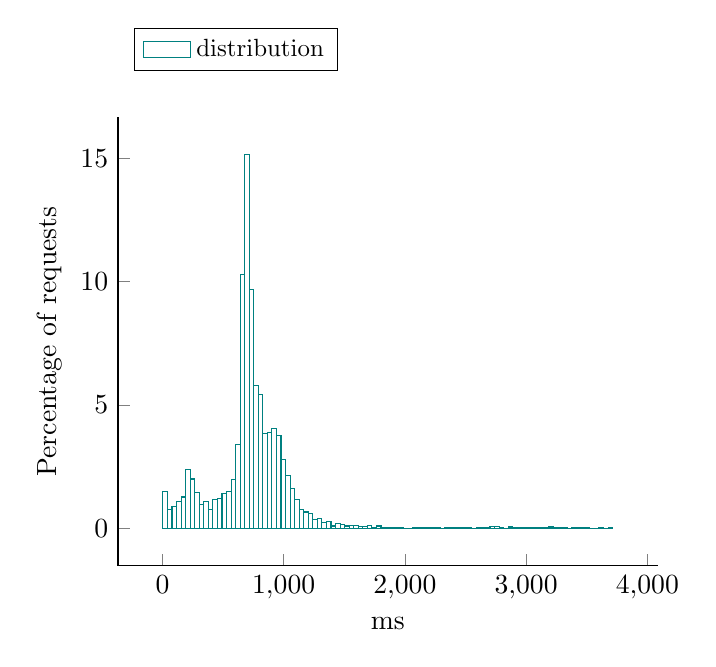
\begin{tikzpicture}
            \begin{axis}[ylabel = Percentage of requests, 
xlabel = ms, 
legend style = {nodes={scale=0.9, transform shape}, at={(0.03,1.2)}, anchor=north west, draw=black, fill=white, align=left, legend columns=3},
area style, mark size = 0pt,
 cycle list name = exotic,
  axis lines* = left]
		\addplot +[ybar interval] coordinates {
			 (4, 1.49577)
			 (41.47, 0.763359)
			 (78.94, 0.887147)
			 (116.41, 1.10378)
			 (153.88, 1.26883)
			 (191.35, 2.38292)
			 (228.82, 2.00124)
			 (266.29, 1.43388)
			 (303.76, 0.979988)
			 (341.23, 1.07283)
			 (378.7, 0.773674)
			 (416.17, 1.15535)
			 (453.64, 1.19662)
			 (491.11, 1.41325)
			 (528.58, 1.47514)
			 (566.05, 1.99092)
			 (603.52, 3.40417)
			 (640.99, 10.3053)
			 (678.46, 15.1537)
			 (715.93, 9.6864)
			 (753.4, 5.78708)
			 (790.87, 5.41572)
			 (828.34, 3.85806)
			 (865.81, 3.86837)
			 (903.28, 4.03342)
			 (940.75, 3.77553)
			 (978.22, 2.77491)
			 (1015.69, 2.13534)
			 (1053.16, 1.60924)
			 (1090.63, 1.17599)
			 (1128.1, 0.763359)
			 (1165.57, 0.660202)
			 (1203.04, 0.598308)
			 (1240.51, 0.371364)
			 (1277.98, 0.391995)
			 (1315.45, 0.247576)
			 (1352.92, 0.257891)
			 (1390.39, 0.0928409)
			 (1427.86, 0.195998)
			 (1465.33, 0.154735)
			 (1502.8, 0.0928409)
			 (1540.27, 0.113472)
			 (1577.74, 0.113472)
			 (1615.21, 0.0825253)
			 (1652.68, 0.0825253)
			 (1690.15, 0.113472)
			 (1727.62, 0.0412626)
			 (1765.09, 0.0928409)
			 (1802.56, 0.0103157)
			 (1840.03, 0.0412626)
			 (1877.5, 0.030947)
			 (1914.97, 0.0206313)
			 (1952.44, 0.0206313)
			 (1989.91, 0)
			 (2027.38, 0)
			 (2064.85, 0.0103157)
			 (2102.32, 0.0206313)
			 (2139.79, 0.0103157)
			 (2177.26, 0.0206313)
			 (2214.73, 0.0206313)
			 (2252.2, 0.030947)
			 (2289.67, 0)
			 (2327.14, 0.0103157)
			 (2364.61, 0.0103157)
			 (2402.08, 0.0206313)
			 (2439.55, 0.0206313)
			 (2477.02, 0.0206313)
			 (2514.49, 0.0103157)
			 (2551.96, 0)
			 (2589.43, 0.0412626)
			 (2626.9, 0.0206313)
			 (2664.37, 0.0206313)
			 (2701.84, 0.0825253)
			 (2739.31, 0.0722096)
			 (2776.78, 0.030947)
			 (2814.25, 0)
			 (2851.72, 0.0515783)
			 (2889.19, 0.0412626)
			 (2926.66, 0.030947)
			 (2964.13, 0.030947)
			 (3001.6, 0.0206313)
			 (3039.07, 0.030947)
			 (3076.54, 0.0206313)
			 (3114.01, 0.0206313)
			 (3151.48, 0.0206313)
			 (3188.95, 0.0515783)
			 (3226.42, 0.030947)
			 (3263.89, 0.030947)
			 (3301.36, 0.030947)
			 (3338.83, 0)
			 (3376.3, 0.0206313)
			 (3413.77, 0.0206313)
			 (3451.24, 0.0206313)
			 (3488.71, 0.0412626)
			 (3526.18, 0)
			 (3563.65, 0)
			 (3601.12, 0.0206313)
			 (3638.59, 0)
			 (3676.06, 0.0103157)
			 (3713.53, 0)
		};
\addlegendentry{distribution};
           \end{axis}
      \end{tikzpicture}
  \end{adjustbox}
  \caption{Response time distribution - req = ReadUser-3}
\end{figure}
\end{minipage}\hfill\begin{minipage}{0.18\linewidth}
\begin{table}[h]
\begin{tabular}{|cc|}
\hline
\textbf{} & \textbf{ms}\\ \hline
 \Xhline{0.005\arrayrulewidth}
min & 4\\
 \Xhline{0.005\arrayrulewidth}
max & 3751\\
 \Xhline{0.005\arrayrulewidth}
mean & 733\\
 \Xhline{0.005\arrayrulewidth}
std & 354\\
\hline
\hline
 \Xhline{0.005\arrayrulewidth}
25th & 642\\
 \Xhline{0.005\arrayrulewidth}
50th & 715\\
 \Xhline{0.005\arrayrulewidth}
75th & 865\\
 \Xhline{0.005\arrayrulewidth}
80th & 911\\
 \Xhline{0.005\arrayrulewidth}
85th & 960\\
 \Xhline{0.005\arrayrulewidth}
90th & 1024\\
 \Xhline{0.005\arrayrulewidth}
95th & 1159\\
 \Xhline{0.005\arrayrulewidth}
99th & 2144\\
\hline
\end{tabular}
\caption{Response time}
\end{table}
\end{minipage}\hfill